\section{Rollenverteilung}
\label{sec:PlanungRollenverteilung}

	\begin{xltabular}{\linewidth}{|l|X|}
		\hline
		\textbf{Rolle} & \textbf{Person}
		\\\hline
		Leiter & Simeon Stix
		\\\hline
		Entwickler & Simeon Stix
		\\\hline
		Betreuer & Sven Nüesch
		\\\hline
	\end{xltabular}
	\label{tab:planungrollenverteilungtable}
	\addcontentsline{lot}{table}{\protect\numberline{\thetable} Rollenverteilung im Projekt CKI}
\section{Aufgabenliste} 
\label{sec:PlanungAufgabenliste} 
\begin{enumerate} 
	\item \textbf{\emph{Planung:}} 
	\begin{itemize} 
		\item Aufgabenliste erstellen
		\item Zeiteinteilung 
		\item Meilensteine definieren 
		\item Gantt erstellen 
	\end{itemize} 
	\item \textbf{\emph{Analyse:}} 
	\begin{itemize} 
		\item Recherche CNN 
		\item Recherche Testdaten 
		\item Recherche C++ Details 
		\item Anforderungen definieren 
		\item Use Cases 
		\item weitere Analysen 
		\item Analyse schreiben
	\end{itemize} 
	\item \textbf{\emph{Design:}} 
	\begin{itemize} 
		\item GUI konzipieren 
		\item Wireframes zeichnen 
		\item Konsolenbefehle definieren 
		\item Konsolen-Output definieren 
	\end{itemize}
	\item \textbf{\emph{Realisation:}} 
	\begin{itemize} 
		\item Input Layer realisieren 
		\item Convolutional Layer realisieren 
		\item Pooling Layer realisieren 
		\item Dense Layer Klasse schreiben 
		\item Output Layer erstellen 
		\item CNN-Model erstellen 
		\item CNN-Model trainieren 
		\item GUI auf CNN-Model setzen 
		\item GPU-Anbindung implementieren 
		\item Kommentare schreiben 
		\item weitere Verbesserungen vornehmen 
		\item Buffer-Zeit fürs Programmieren 
	\end{itemize} 
	\item \textbf{\emph{Dokumentieren:}} 
	\begin{itemize} 
		\item Schreiben 
	\end{itemize} 
	\item \textbf{\emph{Testen:}} 
	\begin{itemize} 
		\item Testliste kreieren 
		\item Tests implementieren 
		\item Tests durchführen 
	\end{itemize} 
	\item \textbf{\emph{Deployment:}} 
	\begin{itemize} 
		\item Projekt als EXE bauen 
		\item Build-Anleitung kreieren 
	\end{itemize} 
	\item \textbf{\emph{Präsentation:}} 
	\begin{itemize} 
		\item Präsentation erstellen 
	\end{itemize}
\end{enumerate} 
\section{Meilensteine} 
\label{sec:PlanungMeilensteine} 

\begin{xltabular}{\linewidth}{|X|X|} 
	\hline Meilenstein-Name & Datum 
	\\\hline Vorbereitungen abgeschlossen & 20.10.2023 
	\\\hline CNN-Model Kreation abgeschlossen & 10.11.2023 
	\\\hline Dokumentation abgeschlossen & 01.12.2023 
	\\\hline Produkt abgeschlossen & 05.01.2024 
	\\\hline Projekt abgeschlossen & 10.02.2024 
	\\\hline \hl{Projekt abgegeben} & \hl{23.02.2024} 
	\\\hline 
\end{xltabular}
\addcontentsline{lot}{table}{\protect\numberline{\thetable}Meilensteine}

\label{tab:PlanungMeilensteineTable}
\section{Gantt} 
\label{sec:PlanungGantt} 
\begin{landscape}
	\addcontentsline{lof}{figure}{\protect\numberline{\thefigure}Das Gantt-Diagramm für das Projekt CKI}
	\begin{figure}[htbp]
		\centering
		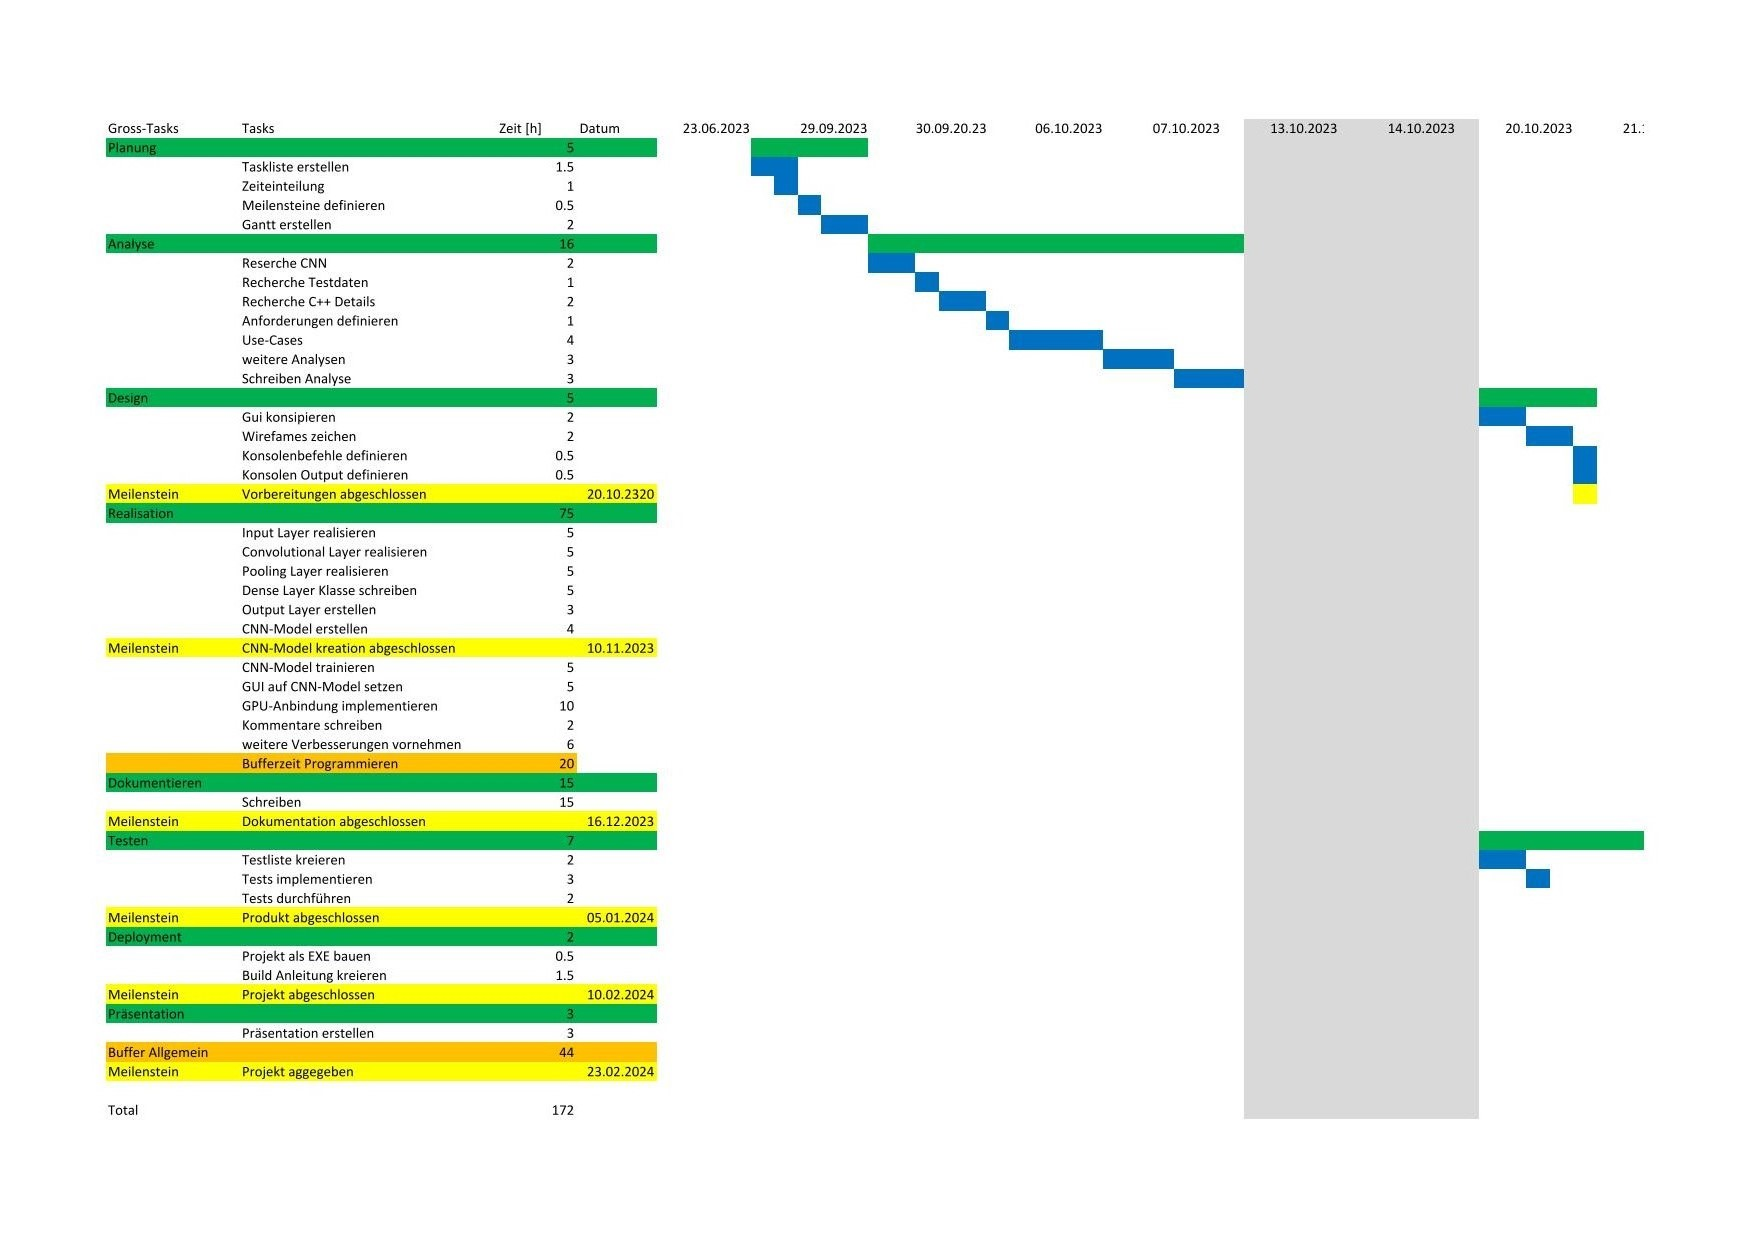
\includegraphics[width=\linewidth, height=\textheight, keepaspectratio]{gantt1_turned.jpg}
		\label{fig:gantt1}
	\end{figure}

	\begin{figure}[htbp]
		\centering
		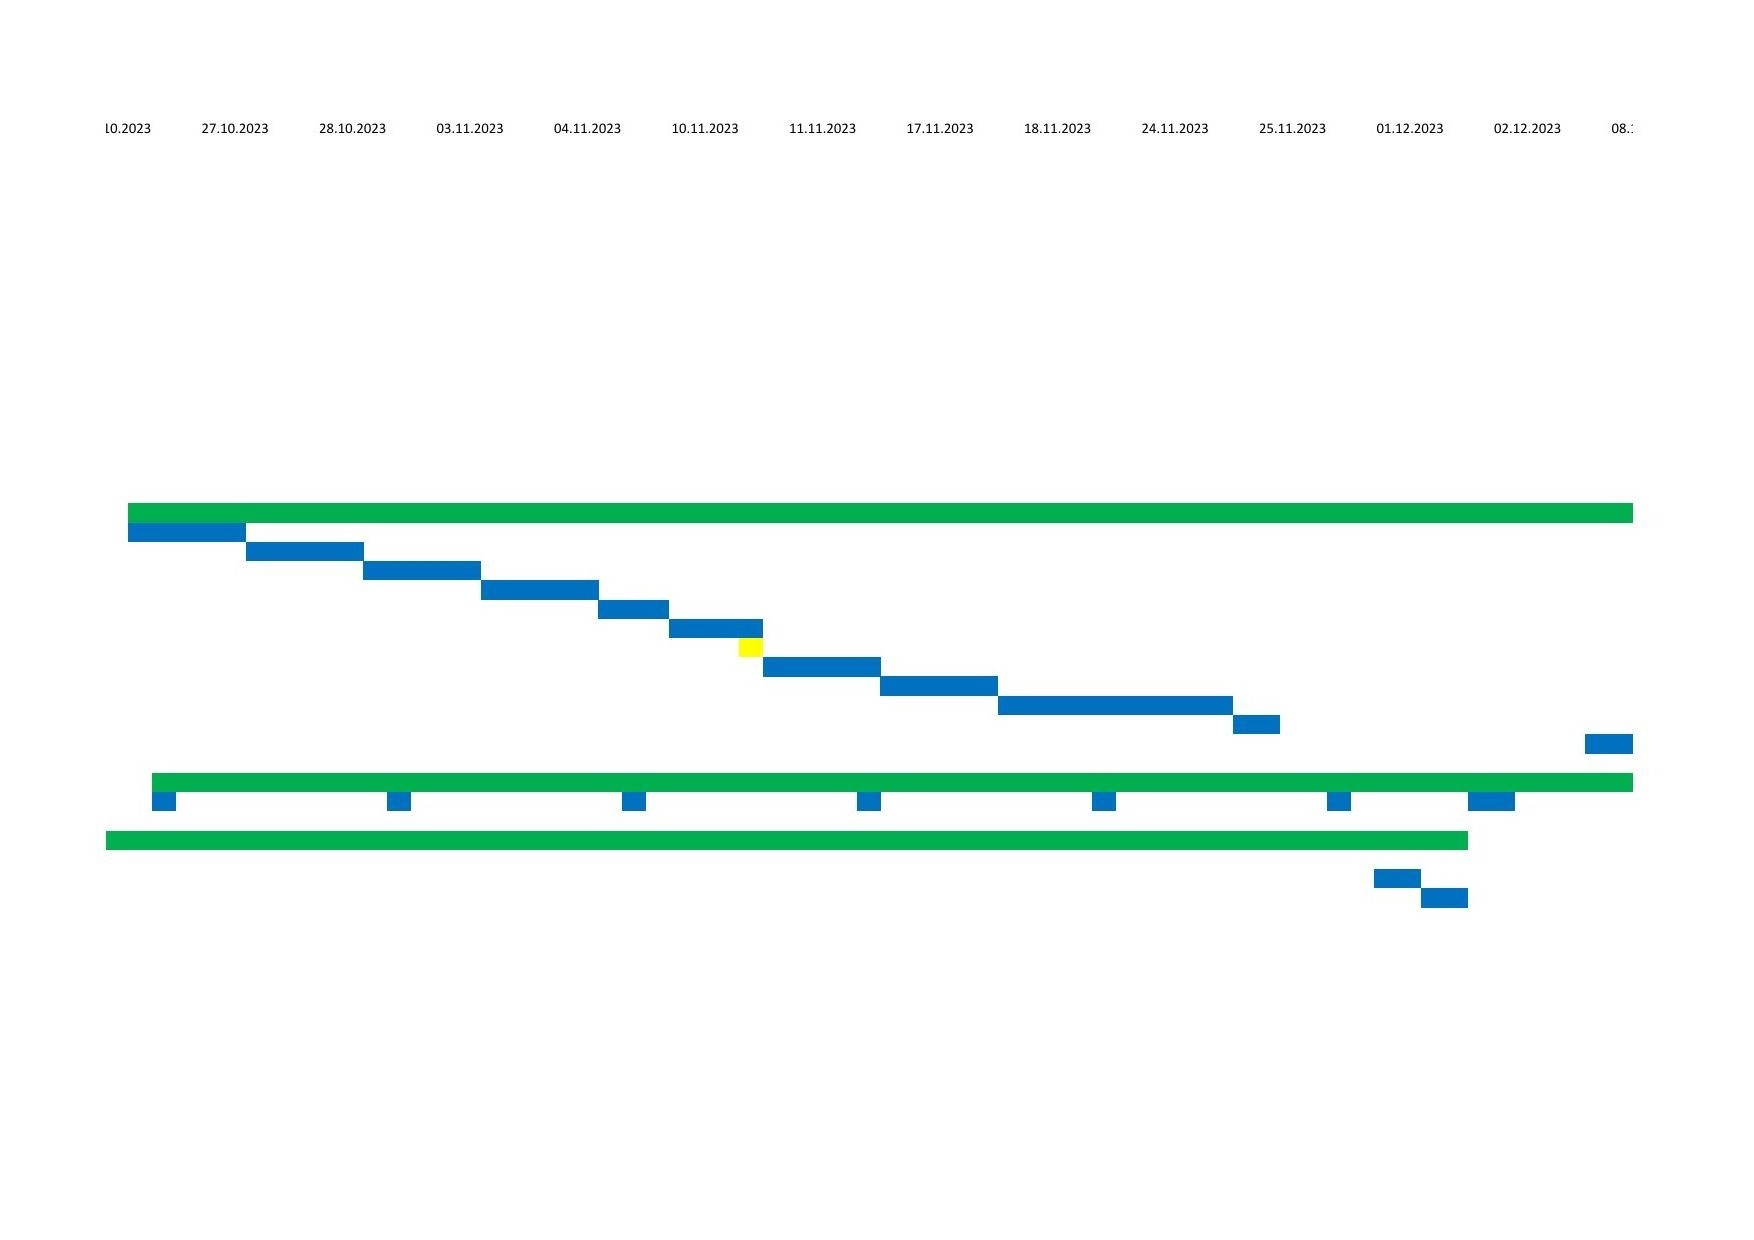
\includegraphics[width=\linewidth, height=\textheight, keepaspectratio]{gantt2_turned.jpg}
		\label{fig:gantt2}
	\end{figure}

	\begin{figure}[htbp]
		\centering
		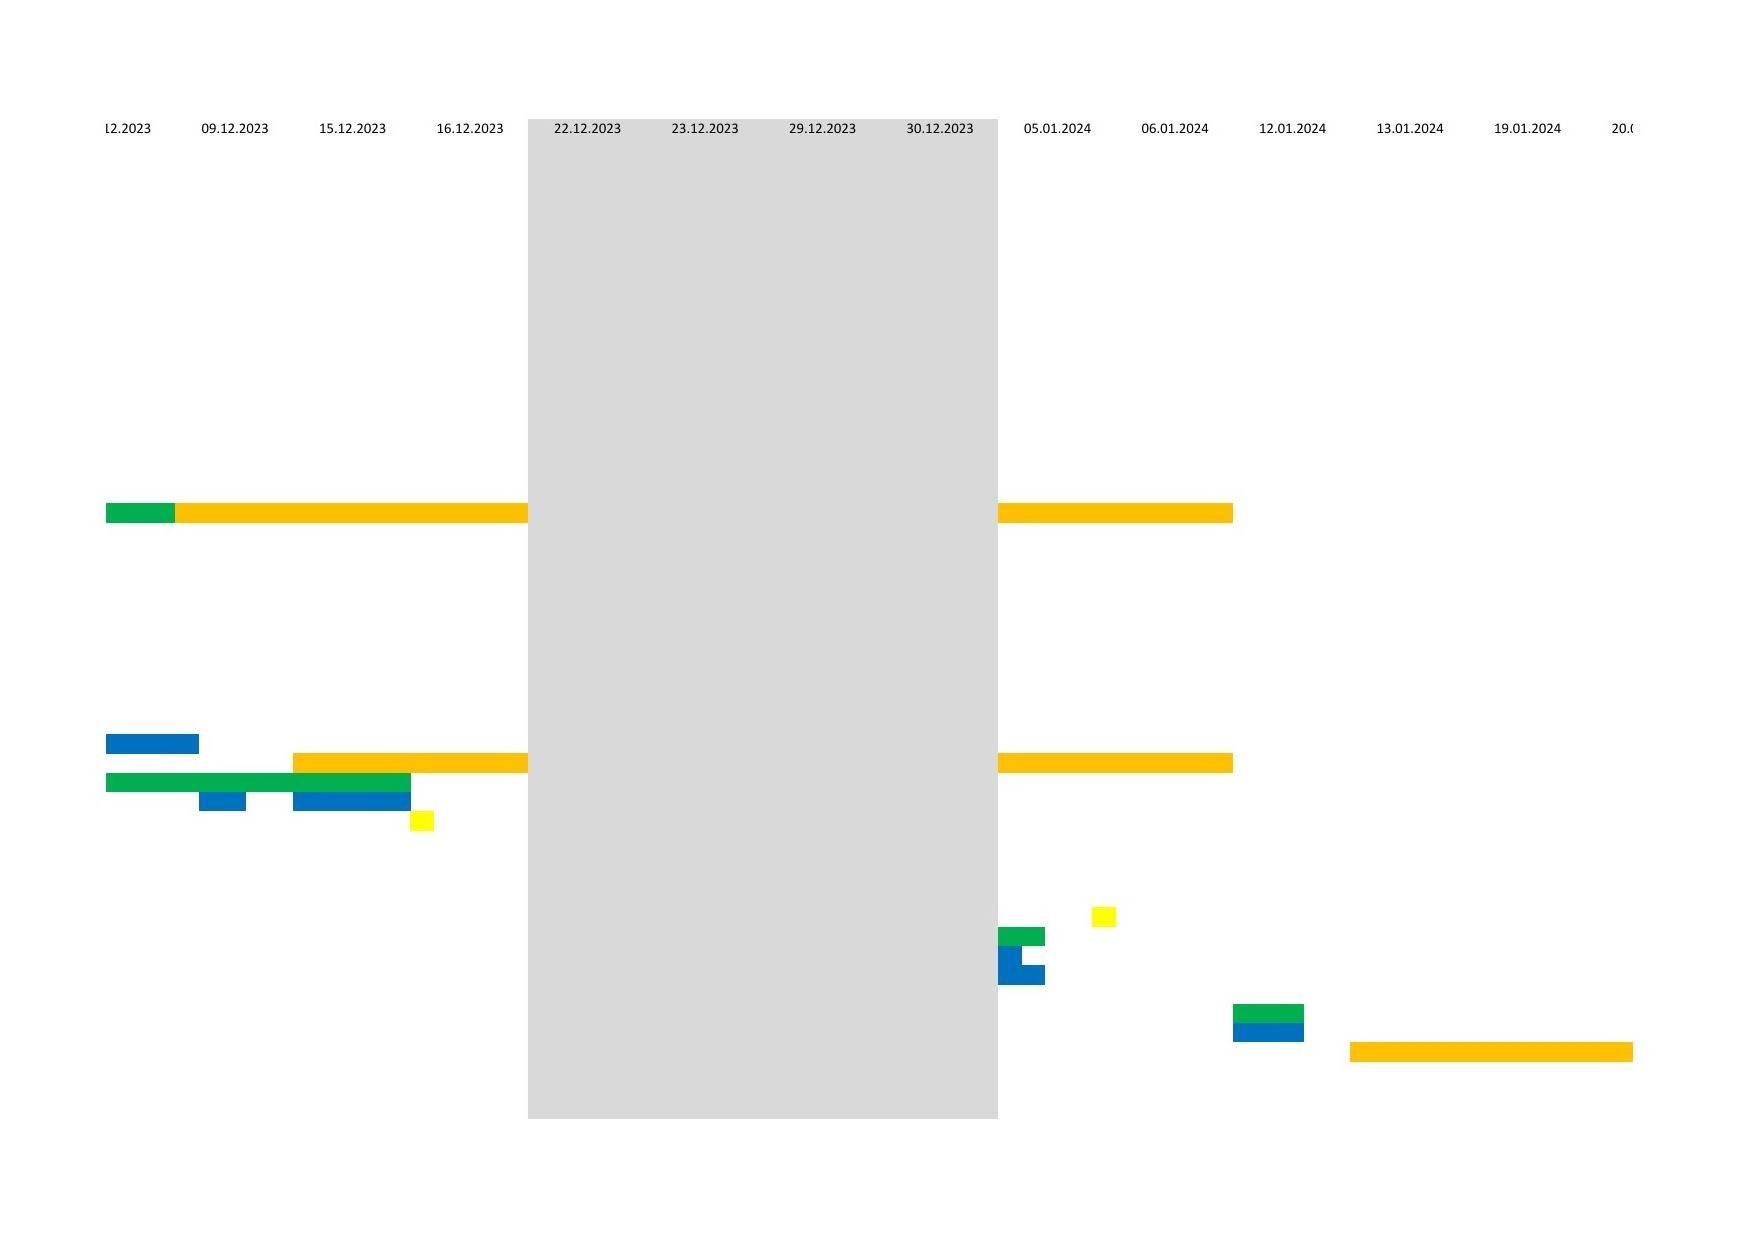
\includegraphics[width=\linewidth, height=\textheight, keepaspectratio]{gantt3_turned.jpg}
		\label{fig:gantt3}
	\end{figure}

	\begin{figure}[htbp]
		\centering
		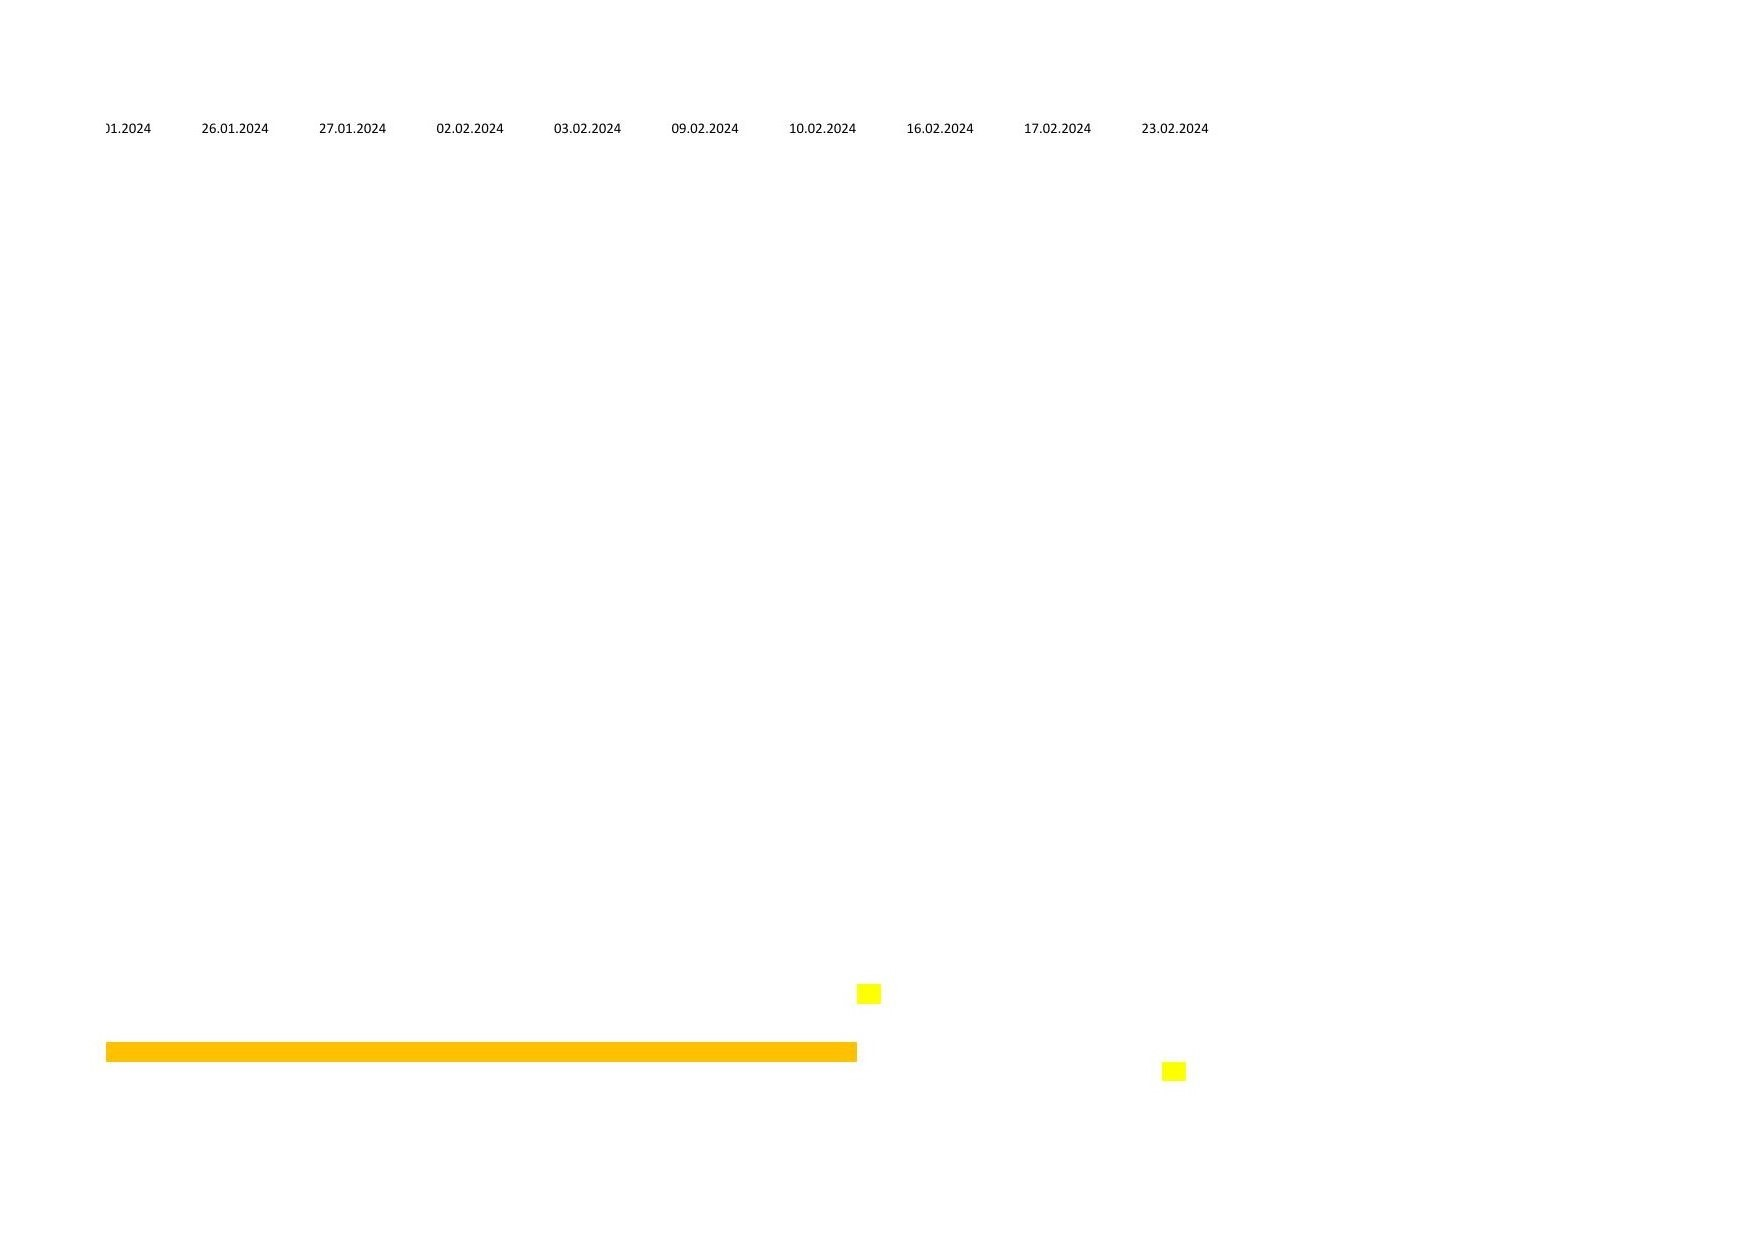
\includegraphics[width=\linewidth, height=\textheight, keepaspectratio]{gantt4_turned.jpg}
		\label{fig:gantt4}
	\end{figure}

\end{landscape}



